\renewcommand*{\arraystretch}{1.1}

\subsection{Interactive / delete / 8}
\label{sec:interactive-delete-08}

% change \emph{} to use sans-serif font
\let\oldemph\emph
\renewcommand{\emph}[1]{{\footnotesize \sf #1}}

\renewcommand{\currentQueryCard}{8}
\marginpar{
	\raggedleft
	\vspace{0.22ex}

	\queryRefCard{interactive-delete-01}{ID}{1}\\
	\queryRefCard{interactive-delete-02}{ID}{2}\\ 
	\queryRefCard{interactive-delete-03}{ID}{3}\\
	\queryRefCard{interactive-delete-04}{ID}{4}\\
	\queryRefCard{interactive-delete-05}{ID}{5}\\
	\queryRefCard{interactive-delete-06}{ID}{6}\\
	\queryRefCard{interactive-delete-07}{ID}{7}\\
	\queryRefCard{interactive-delete-08}{ID}{8}\\
}


\noindent\begin{tabularx}{\queryCardWidth}{|>{\queryPropertyCell}p{\queryPropertyCellWidth}|X|}
	\hline
	query & Interactive / delete / 8 \\ \hline
%
	title & Remove person \\ \hline
%
	% pattern & \centering 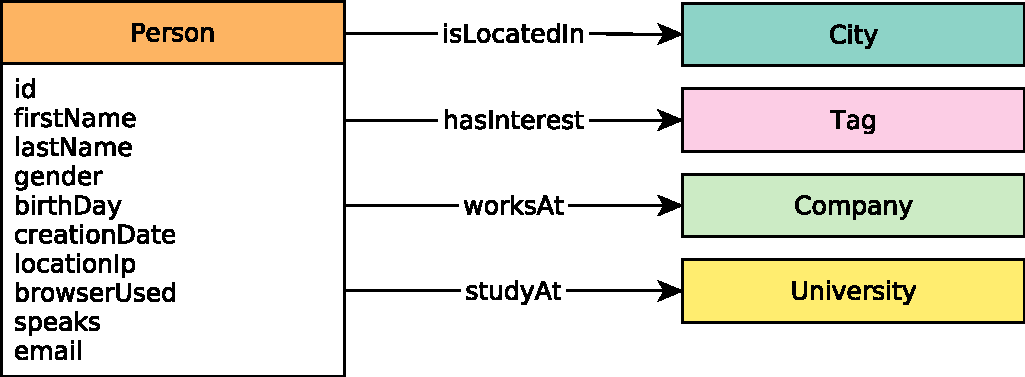
\includegraphics[scale=\patternscale,margin=0cm .2cm]{patterns/interactive-update-01} \tabularnewline \hline
%
	desc. & Remove a \emph{Person} \textbf{node} and it's incident \textbf{edges} (\emph{isLocatedIn}, \emph{studyAt}, \emph{workAt}, \emph{hasInterest}, \emph{likes}, \emph{knows}, \emph{hasMember}, \emph{hasModerator}, \emph{hasCreator}). The removal of a \emph{Person} removes all \emph{Forum} they are moderator of and all messages they have posted in other forums. 

 \\ \hline
%
	
		params &
		\innerCardVSpace{\begin{tabularx}{\attributeCardWidth}{|>{\paramNumberCell}c|>{\varNameCell}M|>{\typeCell}m{\typeWidth}|Y|} \hline
		$\mathsf{1}$ & Person.id
 & ID
 & \texttt{forumId}
 \\ \hline
		\end{tabularx}}\innerCardVSpace \\ \hline
	
%
	
%
	%
	%
	%
	%
\end{tabularx}
\queryCardVSpace

% change \emph back to the old one
\let\emph\oldemph

% Comments/Discussion Points:
% Does deleting a person remove posts/comments they are creator of? Example comment 23 by person X is reply to comment 22 by person Y which is a reply to comment 21 by person Z. Delete person Y, does comment 23 then become a reply to comment 21?  